
\documentclass[]{article}
\usepackage{hyperref}
\usepackage{xcolor}
\usepackage{graphicx}
%\usepackage{package}
%opening
% % % comamnds % % %
\newcommand{\ul}[1]{\underline{#1}}
\renewcommand{\emph}[1]{\textit{#1}}
\newcommand{\important}[1]{\textbf{#1}}
%notes
\newcommand{\notes}[1]{\textcolor{red}{#1}}
\newcommand{\todo}[1]{\textcolor{blue}{#1}}
\newcommand{\idea}[1]{\textcolor{green}{#1}}

\title{Tips and Tricks for WALDORF MicroWave II and the XT Version}
\author{Ameyah and Various}

\begin{document}

\maketitle

\begin{abstract}
	\noindent
	This is a collection notes from various authors on tips and tricks for the Microwave II, so that its possible to quickly print them or have them available for browsing. The author of this document is thankful to the other authors of the quotes here.\\
	\today
\end{abstract}

\section{Introduction}
% !TeX spellcheck = en_US
This little quick tour from here: \href{https://www.carbon111.com/xt_intro.html}{Carbon111}
\subsection{A Quick Tour of the MicrowaveII/XT}
If you need a quick introduction to the Microwave II/XT or just want to know what all the fuss is about, here you go.
Welcome to my quick tour of the Microwave II/XT/XTk (for simplicity's sake hereafter refered to as the XT). If you are familiar with Subtractive Analog synthesis then you will readily understand the XT. First, lets look at a block diagram of how the WaveXT is laid out - this will be our "roadmap":
A complete answer for just reference.
\bigskip % Add an empty line
%These are optional parameters to finetune the placement of tables and figures, with the following meaning:
%
%h, here
%t, top
%b, bottom
%p, page of float
%e.g. \begin{figure}[!htb]
\begin{figure}[ht!]
	\centering
	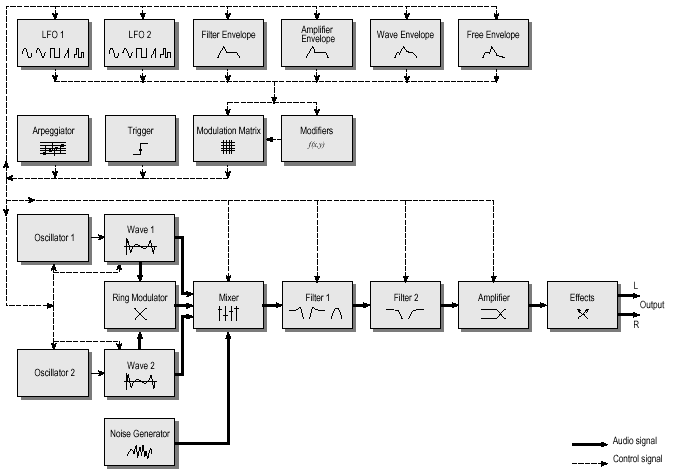
\includegraphics[width=90mm]{pics/mwxt_block.png}
	\caption{Microwave II block diagram}
	\label{blockdiagrammwxt}
\end{figure}
\paragraph{Oscillators and Wavetables}
Our First stop is the Oscillators. The XT has two of these. Unlike a standard analog synthesizer, the oscillators aren't heard directly - they merely drive the frequency of the waveform generators for the currently chosen wavetable. If this doesn't make sense immediately, don't worry about it, just remember that the oscillators drive the pitch of the currently chosen wavetable wave. The oscillators and wavetabes (and, for that matter, even the filters) of this synth make no apologies about being unabashedly digital.\\
Wavetable synthesis is characterized by the ability to sequence through a table of different waveforms during the duration of a single note. The XT has 65 preset wavetables and 32 user-programmable wavetables. A wavetable can be pictured as a row of 64 pointers to any of the 300 waveforms stored in the XT's ROM memory or any waveforms available in the user memory. Lets look at wavetable 016 "Square Saw" as an example:
\begin{figure}[ht!]
	\centering
	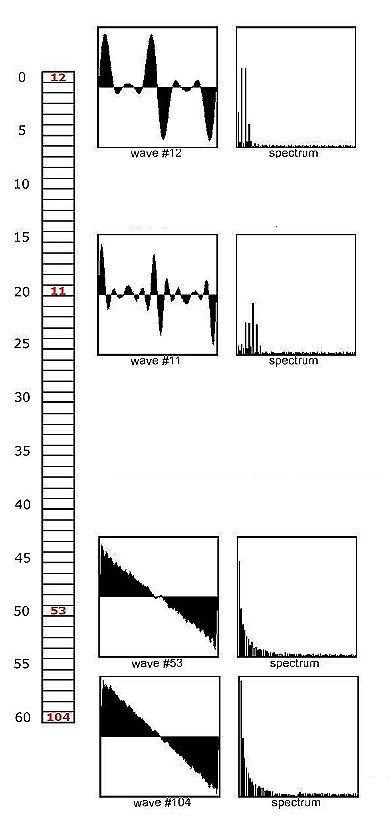
\includegraphics[width=90mm]{pics/osc_wt.jpg}
	\caption{pointers and wavetable with spectrum}
	\label{osc_wt}
\end{figure}
At position 0 is a pointer to ROM waveform \#12, a waveform with strong 2nd and 3rd harmonics, vaguely reminiscent of a square wave. The next pointer is at position 20 for ROM wave \#11, similar to \#12 but with higher harmonics. Next at position 50 is ROM wave \#53, very close to a sawtooth wave. Finally at position 60 is ROM wave \#104, a familiar classic ``buzzy'' sawtooth. The table positions from 1 - 19, 21 - 49 and 51 - 59 are interpolated by the XT automatically. If you move the start wave up or down the wavetable with an envelope, LFO or even the modwheel, you get a smooth transition between each of the four ``real'' waveforms because of the crossfading or "morphing" caused by the XT's interpolation to fill in the gaps.\\
So, if you were to set up a simple sound with just one oscillator with an initial start wave setting of 0 and a basic ramp envelope controlling wavetable position, when you struck a key, you would get a smooth sweep from a ``squarish-sounding'' wave \#12 all the way to a bright "buzzy" sawtooth wave \#103 without any gaps or glitches in between. Of course we are not limited to gentle sweeps with simple ramp EGs - we can use the powerful 8-time 8-level wave envelope generator with its sustain and release loops to create unique and complex timbral morphs if we want - and we do want!\\
The last three positions in each wavetable (61, 62 \& 63) are always reserved for the classic analog subtractive synth waveforms: saw, square and triangle so they are always available if needed. We can turn on a ``limit'' function for the oscillators so we don't unintentionally stray onto the analog waves when scanning the wavetable - a handy feature to avoid timbral glitches. Some of the wavetables in the XT emulate different types of filter sweeps, others offer simulated pulse width modulation, formant sweeps and other timbral morphs. These are designed to be swept with an envelope, LFO or smooth modulator of your choice. Other wavetables like 064 ``Chorus2'' are designed instead to make use of the keytrack parameter to keep a homophonic timbre across a number of octaves - changing the waveform depending on the key played. Still, other wavetables, like the four ``Wavetrip'' tables, are diverse collections of disparate waves well suited to creative cacophony and euphony of all kinds.\\
Hardwired to the wave position parameter of waveform generators 1 and 2 is the so-called wave envelope which is a very powerful 8-time 8-level complex envelope with user-adjustable looping points in the sustain and release segments. This envelope can be used to modulate other elements in the XT too through the modmatrix - more on that later.\\
Ring modulation, hard sync and glide are available for even more oscillator mayhem but lest we dwell too long at the start of our trip we forge on...
\paragraph{Filters}
Next on our journey are the filters. The XT is outfitted with two filters set up in series. The second filter is a basic 6dB filter switchable between lowpass or highpass - mainly used to ``tidy up'' the output of the first filter. The main filter on the XT is an amazing multimode beast with 10 different filter types - lets look at some of the more interesting possibilities:
\begin{itemize}
	\item 24dB and 12dB Lowpass: These are the ``classic'' analog-style filters used for most subtractive synthesis. The 24dB gives an ``aggressive'' filtered sound reminiscent of a Moog ``ladder'' while the 12dB offers a much softer slope much like the old Oberheim synths. Even though the XT is no ``virtual analog'', the filters can be very convincing depending on the application. 
	\item Sine Waveshaper and 12dB Lowpass: This filter packs a real punch with a tight compression sound provided by the sine waveshaper. Excellent on bass sounds.
	\item Waveshaper: This filter has some real suprises, similar to the Sine Waveshaper but with the ability to use any wave in the current wavetable as the shaper wave! Used with a square wave, this filter will rip your face off.
	\item Dual Lowpass/Bandpass: This is a dual filter combining a 12dB lowpass with a 12dB bandpass in series. Sweep different cutoff settings for each filter from different modulators to get amazing shimmering, ``swirling-in-front-of-your-face'' type sounds.
	\item S/H (Sample \& Hold) into 12dB Lowpass: This filter is a brutal sample-rate reduction processor combined with a standard 12dB lowpass. Make the XT sound like a really crappy, cheap low-res sampler! This is a good thing!
	\item There are six other filters as well but I will let you discover those for yourself.
\end{itemize}
Hardwired to the Filter is a basic ADSR envelope that can be used with or overridden by any modulation you choose. Modulating decay time with key velocity is a nice touch for instance.
\paragraph{Amplifier \& Pan}
Pretty basic but you gotta have it. An amp with its own hardwired ADSR feeds directly into a panning circuit. You can modulate pan position with a modulator of your choosing - a random S/H waveform is one of my favorites. Next...
\paragraph{Modulation Matrix}
Here lies the element that pulls all this power into a cohesive force! The modulation matrix allows you to route any of 32 modulation sources to any of 43 destinations! Sources include any of the XT's four envelopes, two LFOs, wheels, pressure, keytrack, etc. Destinations include wave position, pitch, amp levels, LFO rate, volume, panning, cutoff, resonance, you-name-it! You can also do an end-run around any of the XT's hardwiring and, for example, use the wave envelope to control the filter cutoff and the filter envelope to control pan position.
\paragraph{Other}
Yes, I know there's much more - but this was a quick tour, remember. If you still want to know more about the XT, download the User Manual or check out Waldorf's "Additional Information" page. Better yet, try one out! \todo{Add literature references}
\section{Tips and Tricks}
% !TeX spellcheck = en_US
those tips are collected from \href{https://www.carbon111.com/mwxt.html}{Carbon111}
\subsection{An Extra LFO from Modifiers}
A cool way to generate a third LFO to use for that extra touch of animation for your monster sound! Submitted by Rizacan.\\
An extra LFO won't disturb anyone! Here's a little LFO idea using Modifiers as below.
\bigskip % Add an empty line
%These are optional parameters to finetune the placement of tables and figures, with the following meaning:
%
%h, here
%t, top
%b, bottom
%p, page of float
%e.g. \begin{figure}[!htb]
\begin{figure}[ht!]
	\centering
	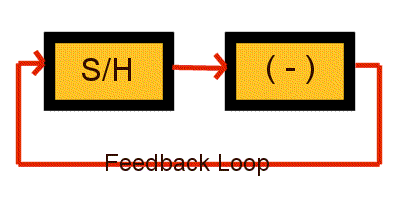
\includegraphics[width=90mm]{pics\lfo_feedback.png}
	\caption{Create a third LFO.}
	\label{third_lfo}
\end{figure}
S/H rate control input sets the overall frequency. Using the filter Modifier, you can get triangle waves. It can also be used for PWM, freeing up other LFOs for other uses!\\
Here are Two examples in Sysex format: \href{https://www.carbon111.com/sysex.zip}{two Examples}
The first one: ``ModifierLFO'' is a simple LFO example. Modifier 1 creates the squarewave and Modifier 3 smoothes the output of Modifier 1 (or 2).\\
The second one, ``Janmichelphaser'', is a simple solina string simulation with a phaser. Modifier 3 produces a triangle waveform using Modifier 1's square wave and modulates PW.
\subsection{Wavetable Browser}
A nice tutorial to create a patch that will allow you to fully audition each of the XT's wavetables. Actually rather handy! Submitted by vanHouten.\\

\section{Information about the wavetables}
% !TeX spellcheck = en_US
This is the description of the PPG Wave 2.2 wavetables as used in the Microwave II/XT. (Plus Wavetable 64).
\begin{itemize}
	\item 001 Resonant: Harmonics 1-8 very strong, simulation of a resonant filter,wave number 00 is a sine wave.
	\item 002 Resonant 2: Similar to wavetable 00, but with additional higher harmonics, dual VCF simulation.
	\item 003 MalletSyn: Similar to two previous wavetables, but also good for vibes, bells, tubular bells, and so on.
	\item 004 Sqr-Sweep: Sine-to-rectangular sweep, low-resonance VCF simulation, clarinette and flute sounds
	\item 005 Bellish: Waves 00-47 feature very high harmonics in progressively greater amplitudes. Waves 47-59 continue to add high harmonics but at a faster rate. Also useful for delay effects and church bells.
	\item 006 Pul-Sweep: Very high harmonics are emphasized, effects similar to wavetable 15, but more mixture-like.
	\item 007 Saw-Sweep: Sine-to-ramp sweep, low-resonance-VCF effects, also good for woodwinds.
	\item 008 MellowSaw: VCF sweep without resonance, also useful for woodwind sounds.
	\item 009 Feedback: Highpass VCF simulation without resonance. Wave 00 has little or no fundamental. Wave 25 has fundamental at maximum amplitude. Useful for dark percussive strings, bass with click-like attack.
	\item 010 Add Harm: Formants are strong middle-range harmonics, useful for ring-modulation and vocal sounds
	\item 011 Reso 3 HP: Similar to wavetable 09.
	\item 012 Wind Syn: Low formants. Wave 00 is dark, 32 is bright, 59 is dark.
	\item 013 High Harm: High formants that sweep.
	\item 014 Clipper: Very strong high-order harmonics, the fundamental is weak. Useful for bright percussive stringed keyboard instrument sounds like clavichord, harpsichord, and so on. When swept, you get an amplitude modulation effect. Wave 00 is maximum amplitude, 24 is minimum amplitude, 59 is maximum. Use great detuning, upper waves and dissonant low chords for noise effects.
	\item 015 Organ Syn: Several organ registers. Sine, Hammond, Lowery, Church organs.
	\item 016 SquareSaw: Harmonics 2 + 3 to sawtooth sweep. Useful for harmonium, accordian, harmonica sounds.
	\item 017 Formant 1: Wild amplitude modulation effects when swept. Several peaks and dips in amplitude.
	\item 018 Polated: Wave 00 features the fundamental and second harmonic. Wave 14 is the fundamental alone. Wave 40 has high harmonics. Wave 59 is the fundamental alone.
	\item 019 Transient: When swept produces high-low-high harmonic sweep effect.
	\item 020 ElectricP: Waves 00-32 are stationary waveforms with string upper harmonics and a few lower harmonics. Wave 59 has no fundamental.
	\item 021 Robotic: Fast discrete changes of low and high harmonics for sample and hold effects. Wave 00 is a sine wave.
	\item 022 StrongHrm: Sine wave to high frequency formants.
	\item 023 PercOrgan: This wavetable is particularly suited for echoing effects. Waveforms vary from original attack plus one delay, to two colored delays. Wave 00 is a sine wave.
	\item 024 ClipSweep: Strong high harmonics.
	\item 025 ResoHarms: Stationary organs. If swept produces ascending high harmonic sweeps.
	\item 026 2 Echoes:	Waves 59 to 49 go from bright to sine wave. 48 to 33 have a colored delay. 33 to 18 are sinewaves. 17 to 00 have a colored delay echo.
	\item 027 Formant 2: Variations on sawtooth waves is strong, bright formants. Good for brass sounds.
	\item 028 FmntVocal: Formant sweeps. When keyboard is used to control the waves vocal and choir sounds can be produced.
	\item 029 MicroSync: Phasing sawtooth waves. Useful for ensemble string sounds.
	\item 030 Micro PWM: Square to rectangular to narrow pulse waves. Sweeps produce pulse-width modulation effects.
	\item 064 Chorus 2: Description by Wolfram Franke (Dec. 1999): "The wavetable is an analysis of a
	male choir sample I did 5 years ago for the Wave. The original choir pitch
	was F 1 and the Wave transformed it so that it generates an equal formant
	spectrum through the whole keyboard range."
\end{itemize}
What about the other ones?
\section{MIDI stuff}
% !TeX spellcheck = en_US
\subsection{Microwave XT Continuous Controllers Chart}
Paul Nagle has graciously granted permission to provide this handy reference chart of MIDI CC numbers and their associated knobs. Great if you want to use the Microwave XT's control surface to manipulate other synths and/or software.\\
\bigskip % Add an empty line
%These are optional parameters to finetune the placement of tables and figures, with the following meaning:
%
%h, here
%t, top
%b, bottom
%p, page of float
%e.g. \begin{figure}[!htb]
\begin{figure}[ht!]
	\centering
	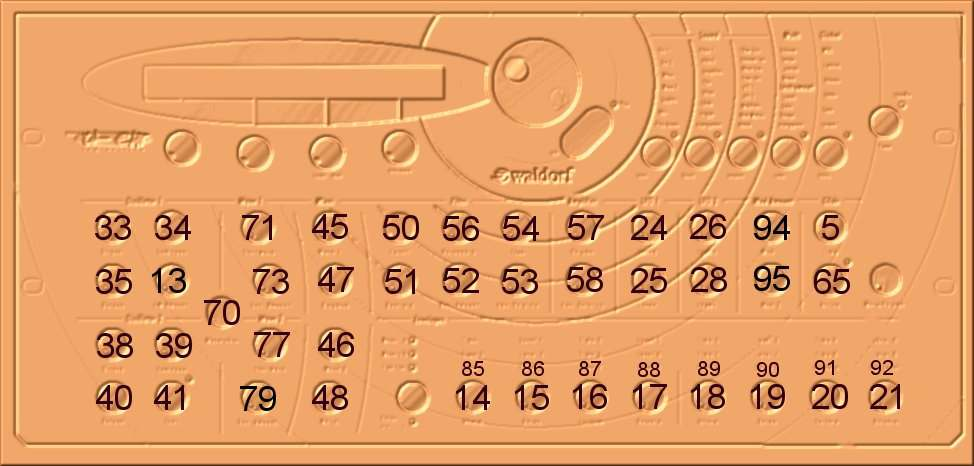
\includegraphics[width=90mm]{pics\xt_midi_chart.jpg}
	\caption{MIDI CC numbers and their associated knobs}
	\label{midi_cc_interface}
\end{figure}
\section{Additional reading material}
% !TeX spellcheck = en_US
%\clearpage
\todo{Not working!}
\bibliography{mwxt} 
%\bibliographystyle{apalike}
\bibliographystyle{alpha}
\end{document}
